\documentclass[aspectratio=169,10pt]{beamer}
\usetheme{default}
\usecolortheme{dove}
\setbeamertemplate{navigation symbols}{}
\usepackage{booktabs}\usepackage{array}
\usepackage[T1]{fontenc}
\usepackage{graphicx}
\usepackage{lmodern}
\setbeamerfont{block body}{size=\small}
\def\evidencetext{}
\setbeamertemplate{footline}{%
  \leavevmode\hbox to \paperwidth{\hspace{0.4cm}\parbox[b]{0.86\paperwidth}{\raggedright\tiny\color{gray}%
  \ifx\evidencetext\empty\else Evidence: \evidencetext\fi}\hfill{\tiny\color{gray}\insertframenumber}\hspace{0.4cm}}\vspace{0.18cm}}
\title{PET final-design selection study}
\subtitle{Study deck (generated from committed results)}
\author{PET final-design study}
\date{\parbox{0.8\linewidth}{\centering\small PET is diagnostic method development. Nothing here is a publication adoption; no historical threshold, verdict or the predecessor campaign's disposition changes; simulation only.}}

\begin{document}

\gdef\evidencetext{}
\frame{\titlepage}

\gdef\evidencetext{\texttt{results/final/decision\_look1.json}; \texttt{results/final/coverage\_dev/coverage\_H2S1T24K5.json}; \texttt{../gbdt\_comparison/results/comparison.json}; \texttt{scalar/results/SCALAR\_AUSSIE\_MATCHED-20260925.json}}
\begin{frame}{What the evidence supports}
{\footnotesize
\begin{tabular}{>{\raggedright\arraybackslash}p{0.30\linewidth}>{\raggedright\arraybackslash}p{0.64\linewidth}}
\toprule
question & what the evidence supports \\
\midrule
Can improved PET recover meaningful physics changes? & \textbf{Yes, in this simulation test.} H2S1T24 $K{=}5$ passed every frozen point-estimator rule: energy tilt 0.895, proton topology 0.391, energy $\times\,q_3$ 0.446. \\
Is it more accurate than GBDT OmniFold? & \textbf{On energy shape, yes; on generator changes, no.} On the same final-bank events PET beats a tuned scalar GBDT OmniFold on the energy tilt (H2S1T24 +0.102, L128S1T24 +0.070 in $R$) but is worse on every generator-model reweighting (NuWro \ensuremath{-}0.247, GiBUU \ensuremath{-}0.206 for H2S1T24). Binned IBU (0.923 on the development tilt) matches PET on the 1D tilt but fails the proton case. \\
Can it give tighter, reliable confidence intervals? & \textbf{Unestablished.} Its six-member bootstrap interval failed calibration: too wide overall (68\,\% intervals cover 0.896), too narrow at low acceptance (0.257). \\
Will it distinguish generators more strongly? & \textbf{Unestablished.} That needs calibrated inference including detector and model uncertainties; no tested procedure provides it, and PET recovers generator-model changes less well than GBDT. \\
\bottomrule
\end{tabular}}\par\vspace{0.15cm}\scriptsize Terminal outcome by the frozen rules: \textbf{NO\_ELIGIBLE\_DESIGN}, no selected default. Signal-only simulation, conditional on the frozen event banks; PET is diagnostic.
\end{frame}

\gdef\evidencetext{\texttt{results/final/decision\_look1.json}; \texttt{results/final/coverage\_dev/decision\_final.json}; \texttt{resources/cost\_fb\_look1-20260930.json}}
\begin{frame}{The two finalists side by side}
{\small
\begin{tabular}{lrr}
\toprule
quantity (final bank, look 1) & H2S1T24 $K{=}5$ & L128S1T24 $K{=}4$ \\
\midrule
Energy-tilt recovery (E0) & 0.895 & 0.863 \\
Proton-topology recovery (E4) & 0.391 & 0.348 \\
Joint energy--momentum-transfer recovery (E5) & 0.446 & 0.450 \\
Estimator-seed spread of energy recovery (N2) & 0.037 & 0.043 \\
Largest observed truth weight (N1) & 90.2 & 33.4 \\
Measured A100-hours per unfolding & 1.77 & 1.52 \\
Frozen point-estimator rules & all pass & B2 fails \\
Interval calibration (coverage) & fails (C1, C4) & not tested (ineligible on B2) \\
\bottomrule
\end{tabular}}\par\vspace{0.15cm}\scriptsize Recoveries: 1 = exact, 0 = no better than the prior. B2's failure is a point decision whose interval crosses the limit; the two designs are not shown to differ in robustness.
\end{frame}

\gdef\evidencetext{\texttt{DEVELOPMENT-20260926.md}; \texttt{PROTOCOL-20260925.md (5)}}
\begin{frame}{Design names}
{\scriptsize
\begin{tabular}{l>{\raggedright\arraybackslash}p{0.80\linewidth}}
\toprule
name part & meaning \\
\midrule
CTL & historical production PET recipe: misses carried, 3 iterations, 8 epochs, forced low rate after iteration 0 \\
C & CTL with the predecessor's efficiency-corrected truth step \\
B & predecessor's feature arm: reco energy summaries at step 1, one-hot particle type at step 2 \\
H1 & C + categorical truth particle type (13-class one-hot) in the truth step \\
H2 & H1 + reco summaries at the detector step (reco $E_\mathrm{avail}$, reco $q_3$, cluster $\Sigma E$ and count) \\
S1 & constant learning rate at every iteration \\
E16 / T24 & 16 epochs per fit at both steps / 24 epochs per truth-step fit \\
L64 / L128 & wider detector-step PET (projection 64 / 128, 4 layers) \\
P2pre / P2scr & Gregor's PET2-small backbone at the detector step on its 33-token typed inputs, pretrained / from scratch \\
A1 & annealed detector-step learning rate after iteration 1 \\
X4 & 4 independently seeded truth-step fits averaged per iteration \\
$K{=}5$, $K{=}4$ & the frozen number of OmniFold iterations \\
\bottomrule
\end{tabular}}\par\vspace{0.1cm}\scriptsize Names compose: H2S1T24 = H2 + S1 + T24. Step 1 reweights simulation to match (pseudo)data at detector level; step 2 turns those weights into truth-level weights; one pass is one iteration.
\end{frame}

\gdef\evidencetext{\texttt{PROTOCOL-20260925.md (3, 4, 6, 9)}}
\begin{frame}{How the numbers are measured}
\small\begin{itemize}
\item \textbf{Simulation only.} Pseudodata are simulated events with a known, injected change to the truth (e.g.\ an
  $E_\mathrm{avail}$ tilt, more protons); the unfolding starts from the unchanged simulation (the prior).
\item \textbf{Recovery} $R = 1 - L_1(\text{unfolded} - \text{target}) / L_1(\text{prior} - \text{target})$ on
  normalized histograms: 1 = the injected change fully recovered, 0 = no better than the prior, $< 0$ = moved away.
\item \textbf{Tests:} energy tilt and its opposite (E0, E3), proton topology (E4, $E_\mathrm{avail} \times$ proton
  class), energy $\times$ momentum transfer (E5), a 21-case robustness library, weight tails and seed spread.
\item \textbf{Fresh events:} designs were developed on a DEV bank; the final test used a bank no earlier work had
  scored, blinded until every final run was complete. A third bank stays sealed.
\item \textbf{Rules frozen first:} every threshold, finalist and sample size was committed before final results were
  seen; the outcome is whatever those rules give.
\item \textbf{Coverage:} does the six-member bootstrap interval contain the true value at its nominal rate across 120
  independent replicates?
\end{itemize}
\end{frame}

\gdef\evidencetext{\texttt{PROTOCOL-20260925.md}}
\begin{frame}{Question, preference and decision rule}
\begin{itemize}\small
\item Select one complete PET design (detector/truth representations, model and initialization, recipe,
  miss rule, iteration count, uncertainty procedure) among a declared, tested family --- or conclude
  ``no eligible design'' / ``unresolved'' with the discriminating evidence.
\item The smaller network is preferred \emph{only} if non-inferior (simultaneous one-sided 95\,\%, margin
  $-0.02$ on the primary recovery, plus frozen regional/topology margins) \emph{and} at least $2\times$
  cheaper in measured total cost; otherwise the stronger larger/pretrained design.
\item Numeric decision table frozen before any successor run (\texttt{PROTOCOL-20260925.md}); final
  inference conditional on frozen event banks; final-bank runs blinded until an explicit UNBLIND
  amendment.
\end{itemize}
\end{frame}

\gdef\evidencetext{\texttt{banks/BANK\_MANIFEST.json}; \texttt{CAPACITY-20260925.md}}
\begin{frame}{Fresh-event capacity and independence}
{\small
\begin{tabular}{lrl}
\toprule
bank & rows & use \\
\midrule
DEV (exposed) & 45089191 & development; every prior \\
FB (never drawn) & 2646891 & final pseudodata; sealed except listed runs \\
RB (pool R, never opened) & 1414846 & reserve; sealed \\
\bottomrule
\end{tabular}}

\vspace{0.3cm}\small Only $\approx 3.4$ historical-size replicates of never-drawn events exist and no further
same-model simulation: final replicates are independent random subsets \emph{given the banks}; the bank's own
offset is reported beside every contrast.
\end{frame}

\gdef\evidencetext{\texttt{results/predecessor\_posthoc/}; \texttt{DIAGNOSTICS-20260925.md}}
\begin{frame}{Where the multiplicity failure sits: the detector step}
\small Injected $E_\mathrm{avail}$ L1: tilt 0.273, protons$\times1.3$ 0.026, neutrons$\times1.3$ 0.011 --- the multiplicity cases barely move the scored marginal.\par\vspace{0.2cm}{\small
\begin{tabular}{lrrrrrr}
\toprule
 & det.\ $\Sigma E$ $k{=}1$ & $k{=}3$ & $k{=}10$ & pull $p$-class $k{=}1$ & $k{=}3$ & $k{=}10$ \\
\midrule
CTL & \ensuremath{-}0.16 & \ensuremath{-}0.37 & \ensuremath{-}0.39 & +0.01 & +0.02 & +0.05 \\
C & \ensuremath{-}0.16 & \ensuremath{-}0.45 & \ensuremath{-}0.44 & +0.01 & +0.03 & +0.08 \\
B & +0.81 & +0.82 & +0.83 & +0.11 & +0.22 & +0.49 \\
\bottomrule
\end{tabular}}\par\vspace{0.2cm}\small Protons$\times1.3$ (2 replicates): the baseline detector step (CTL, C) mis-closes the cluster-energy distribution and transmits almost no proton-content change to the pull; with reco summaries (B) both are transmitted. Development evidence.
\end{frame}

\gdef\evidencetext{\texttt{results/step2int/}; \texttt{DIAGNOSTICS-20260925.md}}
\begin{frame}{Truth-step learnability (bounded interventions)}
{\small
\begin{tabular}{lrrr}
\toprule
truth arm (step 2 on the exact weights) & p-class sel. & p-class missed & n-class sel. \\
\midrule
raw PDG & 0.83 & 0.83 & 0.59 \\
one-hot PDG & 0.87 & 0.88 & 0.88 \\
one-hot + counts & 0.89 & 0.92 & 0.88 \\
one-hot, 24 epochs & 0.97 & 0.96 & 0.98 \\
\bottomrule
\end{tabular}}\par\vspace{0.25cm}\small Given C's real iteration-1 pull, the one-hot truth step recovers 0.012 of the joint $E_\mathrm{avail}\times$proton change; given B's, 0.114. The truth step learns and extrapolates what it receives; the loss is upstream.
\end{frame}

\gdef\evidencetext{\texttt{dev/DEV\_TABLES-20260927.json}; \texttt{DEVELOPMENT-20260926.md}}
\begin{frame}{Development screen (DEV bank)}
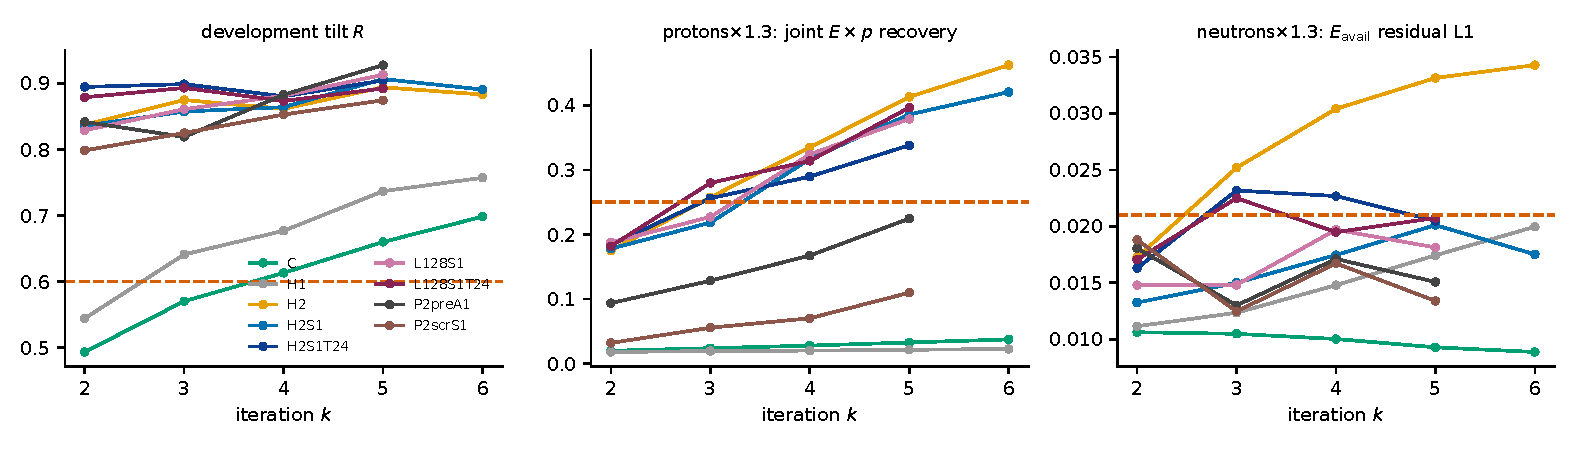
\includegraphics[width=0.95\linewidth]{figures/dev_screen.pdf}\par\small Reco summaries lift the tilt (H2S1 $k{=}5$: 0.906; C $k{=}3$: 0.570); the forced-1e-5 schedule fails the neutron screen (H2 $k{=}3$: 0.025) while the constant rate passes (H2S1 $k{=}5$: 0.020, topology 0.386). Development evidence, 2 draws per case.
\end{frame}

\gdef\evidencetext{\texttt{sizing/n2\_all-20260927-3d.json}; \texttt{PROTOCOL-20260925.md (3b)}}
\begin{frame}{Reproducibility repair (single-unfolding seed spread)}
{\scriptsize
\begin{tabular}{llrrl}
\toprule
design & truth step & $k$ & seed sd of $R_{E0}$ & N2 ($\le 0.05$) \\
\midrule
H2S1 & 8 epochs & 5 & 0.095 & fail \\
L128S1 & 8 epochs & 5 & 0.091 & fail \\
L64S1 & 8 epochs & 4 & 0.057 & fail \\
CS1 & 8 epochs & 6 & 0.054 & fail \\
H2S1E16 & 16 epochs (both steps) & 4 & 0.074 & fail \\
L128S1E16 & 16 epochs (both steps) & 4 & 0.071 & fail \\
H2S1T24 & 24 epochs & 5 & 0.037 & pass \\
L128S1T24 & 24 epochs & 4 & 0.043 & pass \\
\bottomrule
\end{tabular}}\par\vspace{0.2cm}\small DEV draws 0--1 $\times$ 4 estimator seeds at fixed events. The spread sits in the truth step (the detector step varies little with the seed); a 24-epoch truth step repairs it (Amendment 3b).
\end{frame}

\gdef\evidencetext{\texttt{dev/SCREENS-20260927-3d.json}; \texttt{dev/FINALIST\_RULE-20260926.md}}
\begin{frame}{Finalist rule applied mechanically}
{\scriptsize
\begin{tabular}{llrlr}
\toprule
design & $K^*$ & dev.\ tilt at $K^*$ & S-N1 & seed sd (S-N2 $\le 0.05$) \\
\midrule
H2S1T24 & 5 & 0.904 & PASS & 0.037 \\
H2S1 & 5 & 0.906 & PASS & 0.095 \\
H2S1E16 & 4 & 0.881 & PASS & 0.074 \\
CS1 & 6 & 0.680 & PASS & 0.054 \\
L128S1T24 & 4 & 0.873 & PASS & 0.043 \\
L128S1 & 5 & 0.913 & PASS & 0.091 \\
L128S1E16 & 4 & 0.875 & PASS & 0.071 \\
L64S1 & 4 & 0.882 & PASS & 0.057 \\
P2preS1 & 4 & 0.905 & fail & --- \\
P2preA1 & --- & --- & --- & --- \\
P2scrS1 & --- & --- & --- & --- \\
\bottomrule
\end{tabular}}\par\vspace{0.2cm}\small Rule committed before the recoveries it ranks were inspected, with addenda (completeness, S-N1, S-N2); finalists: compact H2S1T24 $K{=}5$, large L128S1T24 $K{=}4$ (Amendments 3c, 3d).
\end{frame}

\gdef\evidencetext{\texttt{scalar/results/SCALAR\_AUSSIE\_MATCHED-20260925.json}; \texttt{scalar/SCALAR\_AUSSIE\_MATCHED-20260925.md}}
\begin{frame}{Algorithmic alternative: AUSSIE (scalar, matched)}
{\scriptsize
\begin{tabular}{lrrrr}
\toprule
AUSSIE setting vs OmniFold $k{=}3$ & moves-away: AUSSIE & OmniFold & worst $R$: AUSSIE & OmniFold \\
\midrule
$\lambda{=}1000$, misses carried, kinematics & 11 & 6 & \ensuremath{-}1.077 & \ensuremath{-}0.217 \\
$\lambda{=}1000$, misses carried, kinematics + species & 8 & 6 & \ensuremath{-}0.985 & \ensuremath{-}0.230 \\
$\lambda{=}0$, efficiency-corrected, kinematics & 14 & 6 & \ensuremath{-}3.876 & \ensuremath{-}0.392 \\
$\lambda{=}0$, efficiency-corrected, kinematics + species & 7 & 6 & \ensuremath{-}0.735 & \ensuremath{-}0.352 \\
\bottomrule
\end{tabular}}\par\vspace{0.2cm}\small Bounded matched stress test (same scalar inputs, miss handling, data and tuning opportunity); truth kinematics $= (E_\mathrm{avail}, p_T, p_\parallel, q_3)$. 12 comparisons: 2 miss rules $\times$ 2 truth-input sets $\times$ 3 OmniFold operating points (shown: $k{=}3$). AUSSIE wins none of the 12 on robustness or stability, so it does not advance to a PET backbone.
\end{frame}

\gdef\evidencetext{\texttt{resources/cost\_t24-20260927.json}; \texttt{sizing/sizing\_final-20260927.json}; \texttt{sizing/sizing\_library-20260927.json}; \texttt{PROTOCOL-20260925.md (3c--3f)}}
\begin{frame}{Frozen finalists and final-stage design}
\small\begin{itemize}\item Compact \textbf{H2S1T24} ($K{=}5$) and large \textbf{L128S1T24} ($K{=}4$): detector reco summaries, categorical truth PDG, constant rate, 24-epoch truth step; step-1 PET 47\,k vs 0.97\,M parameters. Anchors CTL and C at $k{=}3$.\item Cost per unfolding (charged A100-h, declared packing): 1.77 (compact) vs 1.49 (large): the smaller network is not cheaper, so the cost-based preference cannot apply.\item Independent sizing: $n_F = 60$ (capped; $E_0$ non-inferiority between the finalists would need 250 draws --- a quantified limit); D4c/D3 draws 40.\item Final bank: FINAL, 21-case library and coverage run blinded until the UNBLIND amendment.\end{itemize}
\end{frame}

\gdef\evidencetext{\texttt{results/final/decision\_look1.json}; \texttt{resources/cost\_fb\_look1-20260930.json}}
\begin{frame}{Look 1: finalists on the final bank}
{\scriptsize
\begin{tabular}{lrr}
\toprule
look 1 (mean, simultaneous LB) & H2S1T24 $K{=}5$ & L128S1T24 $K{=}4$ \\
\midrule
$E_0$ development tilt (U1) & 0.895 (0.876) & 0.863 (0.842) \\
moderate / good region (U2b) & 0.874 / 0.917 & 0.846 / 0.910 \\
$E_3$ opposite tilt (U3) & 0.835 (0.815) & 0.829 (0.809) \\
$E_4$ proton topology (U4) & 0.391 (0.368) & 0.348 (0.326) \\
$E_5$ $E_\mathrm{avail}\times q_3$ (U5) & 0.446 (0.429) & 0.450 (0.435) \\
N2 seed sd ($\le 0.05$) & 0.037 & 0.043 \\
gain over CTL in $R_{E_0}$ & +0.589 (0.568) & +0.557 (0.535) \\
cost per unfolding (A100-h) & 1.77 & 1.52 \\
status (rules) & INCOMPLETE (C1--C5) & INELIGIBLE (B2) \\
\bottomrule
\end{tabular}}\par\vspace{0.15cm}\small Ranking: CONTINUE (candidates pending: H2S1T24K5). No look 2 (no sequential rule returned CONTINUE). Coverage of H2S1T24 runs blinded.
\end{frame}

\gdef\evidencetext{\texttt{results/final/decision\_look1.json}; \texttt{results/final/b1\_dependence\_look1.json}; \texttt{results/final/population\_look1.json}}
\begin{frame}{Look 1: what the verdict does and does not show}
\small\begin{itemize}\item \textbf{B2} (D4d n down, mean residual $-$ injected $E_\mathrm{avail}$ L1, limit 0.010, a point rule): H2S1T24 0.0097 [0.0025, 0.0169] PASS; L128S1T24 0.0122 [0.0064, 0.0181] FAIL. \textbf{Point-decided, statistically unresolved}: both intervals cross the limit; the difference is not resolved by this comparison. Not evidence that the compact design is more robust, nor that the two are equivalent.\item \textbf{B1} PASSes under its frozen independence-based bound. Under within-draw dependence the evidence is insufficient to establish a per-unit failure probability $\le 0.10$: on the common panel (FB0--7) H2S1T24 has 2/8 draws with a failure (CP upper 0.651), L128S1T24 1/8; with none the bound would be 0.369. This does not show the probability exceeds 0.10.\item Like-for-like and FB-population recoveries agree on the designated endpoints (report \S6, report only).\end{itemize}
\end{frame}

\gdef\evidencetext{\texttt{results/final/coverage\_dev/coverage\_H2S1T24K5.json}}
\begin{frame}{Uncertainty calibration: coverage of H2S1T24}
{\scriptsize
\begin{tabular}{llr}
\toprule
H2S1T24 $K{=}5$, B = 6, 120 replicates & measured & verdict \\
\midrule
C1 pooled 95\,\% (LB $\ge$0.90, point $\le$0.99) & 0.990 (LB 0.980) & unresolved \\
C1 pooled 68\,\% (LB $\ge$0.60, point $\le$0.80) & 0.896 (LB 0.858) & decisive \\
\textbf{C1} (both levels) &  & FAIL \\
C2 every bin 95\,\% $\ge$ 0.85 & all bins pass & PASS \\
C3 moderate / good 95\,\% LB $\ge$ 0.85 & 0.949 / 0.993 & PASS \\
C4 half-width / limit, bins 1--6 ($\le$1) & 1.32--1.72 & FAIL \\
C5 D4c up & skipped after decisive C1--C4 FAIL & --- \\
\bottomrule
\end{tabular}}\par\vspace{0.15cm}\small In aggregate the six-member interval is \textbf{too wide}; the same against the FB population target. Not uniformly conservative: the low-acceptance region \textbf{under-covers} (68\,\%: 0.26, 95\,\%: 0.79), a region no rule gates. Mechanism not established.
\end{frame}

\gdef\evidencetext{\texttt{../gbdt\_comparison/results/comparison.json}; \texttt{../gbdt\_comparison/REPORT-20261005.md}}
\begin{frame}{PET vs GBDT OmniFold on the same events}
{\scriptsize
\begin{tabular}{lll}
\toprule
paired difference in $R$, PET $-$ GBDT & H2S1T24 $K{=}5$ & L128S1T24 $K{=}4$ \\
\midrule
energy tilt E0 (60 draws) & +0.102 [0.084, 0.119] & +0.070 [0.051, 0.089] \\
opposite tilt E3 (60) & +0.076 [0.059, 0.093] & +0.070 [0.053, 0.088] \\
proton topology E4 (40) & +0.055 [0.035, 0.075] & +0.012 [\ensuremath{-}0.007, 0.031] \\
\quad E4 against GBDT run to $k{=}10$ & +0.009 [\ensuremath{-}0.012, 0.030] & \ensuremath{-}0.034 [\ensuremath{-}0.054, \ensuremath{-}0.015] \\
energy $\times\,q_3$ E5 (40) & +0.009 [\ensuremath{-}0.009, 0.026] & +0.013 [\ensuremath{-}0.005, 0.030] \\
generator reweighting: NuWro (8) & \ensuremath{-}0.247 [\ensuremath{-}0.345, \ensuremath{-}0.148] & \ensuremath{-}0.208 [\ensuremath{-}0.324, \ensuremath{-}0.092] \\
\quad NuWro$'$ (8) & \ensuremath{-}0.216 [\ensuremath{-}0.303, \ensuremath{-}0.130] & \ensuremath{-}0.180 [\ensuremath{-}0.241, \ensuremath{-}0.118] \\
\quad GiBUU (8) & \ensuremath{-}0.206 [\ensuremath{-}0.305, \ensuremath{-}0.107] & \ensuremath{-}0.121 [\ensuremath{-}0.177, \ensuremath{-}0.065] \\
\bottomrule
\end{tabular}}\par\vspace{0.12cm}{\scriptsize
\begin{tabular}{lrrr}
\toprule
same draws & H2S1T24 & L128S1T24 & GBDT \\
\midrule
B2 residual, D4d n down (PET rule $\le 0.010$) & 0.0097 & 0.0122 & 0.0033 \\
largest truth weight & 90.2 & 33.4 & 5.6 \\
GBDT's E0 summed per-bin MSE relative to PET & 2.9\ensuremath{\times} & 1.9\ensuremath{\times} & 1 \\
\bottomrule
\end{tabular}}\par\vspace{0.1cm}\tiny GBDT = the matched study's tuned scalar OmniFold (HistGradientBoosting, efficiency-corrected, reco summaries + muon kinematics, truth with species counts, $k{=}7$ chosen on DEV), run on the same look-1 final-bank units with the same events, targets and scorer. Unadjusted 95\,\% intervals; exploratory. GBDT error is mostly systematic under-correction. No uncertainty comparison: this GBDT has no interval procedure here. On DEV, binned IBU and AUSSIE match PET on the 1D tilt and fail hadron or generator cases.
\end{frame}

\gdef\evidencetext{\texttt{results/final/coverage\_dev/decision\_final.json}; \texttt{DECISION\_RECORD-pet-final-design.md}}
\begin{frame}{Terminal outcome (frozen rules)}
\centering\Large\textbf{NO\_ELIGIBLE\_DESIGN}\par\vspace{0.3cm}{\small
\begin{tabular}{ll}
\toprule
finalist & status (rules) \\
\midrule
H2S1T24K5 & INELIGIBLE (C1, C4) \\
L128S1T24K4 & INELIGIBLE (B2) \\
\bottomrule
\end{tabular}}\raggedright\par\vspace{0.3cm}\small\begin{itemize}\item No design selected and no default named (the default must itself be eligible).\item Supported: H2S1T24's point estimator passes every accuracy, robustness and stability rule; its interval procedure fails calibration (too wide in aggregate; under-covers at low acceptance). Not supported: a ranking of the finalists.\item Remaining route (owner decision): \S11 repair --- interval calibrated on DEV, re-validated on the sealed RB bank.\end{itemize}
\end{frame}

\gdef\evidencetext{\texttt{dev/SCREENS-20260927-3d.json}; \texttt{results/final/coverage\_dev/decision\_final.json}; \texttt{DEVELOPMENT-20260926.md}; \texttt{nd-unfolding/pet/configuration\_comparison/CONFIGURATION\_COMPARISON-20260918.md (Gregor's minerva-ml pinned at fc9a099; sections cited as cmp)}}
\begin{frame}{Architectures tested, what came from Gregor's work, and why none passed}
{\tiny
\begin{tabular}{llll}
\toprule
design & change & from Gregor's work & why it did not pass \\
\midrule
H1 & C + categorical truth PDG (13-way one-hot) & type encoding (cmp 2), padding kept distinct; truth step is ours & S-U4 fails at every $k$ (best 0.023; need $\ge$ 0.25) \\
H2 & H1 + reco summaries at step 1 & whole-event energy sums + overflow (cmp 4, 6; not per-family) & no $k$ passes all four screens \\
CS1 & C + constant rate & --- & S-N2 seed sd 0.054 $> 0.05$ \\
H2S1 & H2 + constant rate & as H2 & S-N2 seed sd 0.095 $> 0.05$ \\
H2S1E16 & H2S1, 16 epochs & as H2 & S-N2 seed sd 0.074 $> 0.05$ \\
L64H2 & H2, step-1 PET width 64 & as H2 + one capacity step (cmp 7) & no $k$ passes all four screens \\
L128H2 & H2, step-1 PET width 128 & as H2 + one capacity step (cmp 7) & no $k$ passes all four screens \\
L64S1 & H2S1, width 64 & as L64H2 & S-N2 seed sd 0.057 $> 0.05$ \\
L128S1 & H2S1, width 128 & as L128H2 & S-N2 seed sd 0.091 $> 0.05$ \\
L128S1E16 & L128S1, 16 epochs & as L128H2 & S-N2 seed sd 0.071 $> 0.05$ \\
P2preS1 & PET2-small at step 1, pretrained & his backbone, checkpoint, 33-token typed inputs, recipe & S-N1 step-1 weight tail at $K^*=4$ \\
P2scrS1 & PET2-small, random init & as P2preS1 without the checkpoint & S-U4 fails at every $k$ (best 0.110; need $\ge$ 0.25) \\
P2preA1 & P2preS1, annealed step-1 rate & as P2preS1 & S-U4 fails at every $k$ (best 0.225; need $\ge$ 0.25) \\
P2scrA1 & P2scrS1, annealed step-1 rate & as P2scrS1 & S-U4 fails at every $k$ (best 0.060; need $\ge$ 0.25) \\
H2S1T24 & H2S1, 24-epoch truth step (finalist) & as H2 & final bank: coverage C1, C4 FAIL --- INELIGIBLE (C1, C4) \\
L128S1T24 & L128S1, 24-epoch truth step (finalist) & as L128H2 & final bank: B2 FAIL (point-decided) --- INELIGIBLE (B2) \\
\bottomrule
\end{tabular}}\par\vspace{0.1cm}\tiny Also closed: the step-2 ensemble fallback (H2S1X4, L128S1X4; entry condition never met) and AUSSIE (bounded matched scalar test). Anchors/controls (CTL, C, B) are not selectable. Development screens: S-U1 tilt, S-U3 opposite tilt, S-U4 proton topology, S-B2 D4d residual; then S-N1, S-N2. Gregor-derived parts follow the pinned comparison (cmp sections); the truth-step design is the study's own.
\end{frame}

\gdef\evidencetext{\texttt{results/final/population\_look1.json}; \texttt{dev/SCREENS-20260927-3d.json}; \texttt{scalar/results/SCALAR\_AUSSIE\_MATCHED-20260925.json}; \texttt{../configuration\_comparison/campaign\_report.json}; \texttt{scalar/SCALAR\_AUSSIE\_MATCHED-20260925.md}}
\begin{frame}{Reference methods and alternatives}
{\scriptsize
\begin{tabular}{l>{\raggedright\arraybackslash}p{0.25\linewidth}>{\raggedright\arraybackslash}p{0.12\linewidth}>{\raggedright\arraybackslash}p{0.37\linewidth}}
\toprule
method & what it is & from Gregor's work & result \\
\midrule
CTL $K{=}3$ & historical production PET recipe (anchor) & --- & final bank energy tilt 0.306 (floor 0.556) \\
C $K{=}3$ & efficiency-corrected truth step (anchor) & --- & final bank energy tilt 0.560 \\
B & predecessor's feature arm (control) & energy sums (cmp 4) & development tilt 0.474 at $k{=}3$ \\
Gregor's arm & his PET2-small, his tokens, pretrained; historical comparison, $k{=}3$ & his configuration (adapted) & 0.417 vs ours 0.304; floor 0.556: \textsc{neither eligible} \\
GBDT OmniFold & scalar HistGradientBoosting on reco $p_T$, $p_\parallel$, $E_\mathrm{avail}$, $q_3$, cluster sums & --- & development tilt 0.783 (efficiency-corrected) / 0.418 (misses carried), $k{=}3$; proton topology 0.389 only with species-count truth inputs \\
binned IBU & response-matrix unfolding, efficiency-corrected & --- & development tilt 0.923; moves away in the proton case (\ensuremath{-}0.381) \\
AUSSIE & scalar method of arXiv:2602.24282, matched to GBDT OmniFold & --- & lost all 12 matched comparisons on robustness and stability \\
\bottomrule
\end{tabular}}\par\vspace{0.1cm}\tiny Anchors are not selectable; scalar references use the predecessor's DEV-bank selections, so they are context, not matched comparisons with the PET finalists.
\end{frame}

\gdef\evidencetext{\texttt{docs/orchestration/AUTHORIZATION-20260925-pet-final-design.md}}
\begin{frame}{What this study cannot authorize}
\small\begin{itemize}
\item No publication adoption; no real-data unfolding; no \texttt{C\_stat}/\texttt{C\_ML}; no Gate-6 work;
  \texttt{OI-126} not reopened; the scalar-5D covariance unchanged; no note/primer/paper change.
\item Historical thresholds and verdicts (\texttt{NEITHER\_ELIGIBLE / NO\_SELECTION}) and the predecessor's
  disposition are unchanged.
\item Scope of any selection: signal-only simulation, the inventory's simulated detector response, the study's
  event scale, conditional on the frozen banks; generator dependence beyond histogram reweightings is unprobed.
\end{itemize}
\end{frame}

\end{document}
